\section{sysinfo.c}
Để thu thập thông tin về tài nguyên hệ thống đang hoạt động, nhóm thiết lập thêm một system call mới với mã định danh 
\code{SYS\_sysinfo = 24} trong file \texttt{kernel/syscall.h} \cite{hcmus_os_lab2}. Lời gọi hệ thống này nhận 
vào một đối số duy nhất là con trỏ trỏ tới cấu trúc \code{struct sysinfo} được định nghĩa trong file \texttt{kernel/sysinfo.h}, 
bao gồm $2$ trường dữ liệu chính: \code{freemem} (tổng dung lượng bộ nhớ vật lý còn trống tính theo byte) và \code{nproc} 
(số lượng tiến trình có trạng thái khác \code{UNUSED}). Kernel có nhiệm vụ truy xuất các cấu trúc dữ liệu nội bộ để tính toán 
chính xác hai thông số này và sao chép an toàn về không gian người dùng.

\subsection{Triển khai}
Để thực hiện việc thu thập dữ liệu nhất quán và hiệu quả, nhóm chia
tiến trình xử lý thành ba thành phần: điều phối tiếp nhận tại \texttt{sysproc.c},
đo lường bộ nhớ tự do trong \texttt{kalloc.c}, và đếm số lượng tiến trình còn sống
trong \texttt{proc.c}. Đầu tiên, khi chương trình người dùng phát động lời gọi \code{sysinfo(\&info)},
kernel tiếp nhận yêu cầu tại hàm \code{sys\_sysinfo(void)} nằm trong
\texttt{kernel/sysproc.c}. Tại đây, kernel sử dụng hàm trợ giúp \code{argaddr(0, \&uaddr)}
để trích xuất địa chỉ ảo của vùng nhớ đệm do user cung cấp. Sau đó, hàm lần lượt
gọi hai hàm chuyên trách là \code{count\_freemem()} và \code{count\_proc()} để
điền dữ liệu vào biến tạm \code{info} cục bộ trên Kernel Stack.

Quá trình tính toán lượng bộ nhớ trống được hiện thực trong hàm \code{count\_freemem()}
tại \texttt{kernel/kalloc.c}. Trong hệ điều hành xv6, toàn bộ bộ nhớ vật lý sau
điểm kết thúc của kernel (\code{end}) đến giới hạn \code{PHYSTOP} ($128$ MB) được
quản lý dưới dạng một danh sách liên kết đơn các trang nhớ tự do \code{kmem.freelist}.
Mỗi phần tử trong danh sách này tương ứng với một khung trang (Page Frame) có kích
thước cố định \code{PGSIZE = 4096} byte. Do đó, hàm \code{count\_freemem()} duyệt qua
toàn bộ danh sách liên kết để đếm số lượng trang trống khả dụng, sau đó nhân với
\code{PGSIZE} để quy đổi ra tổng số byte còn rảnh. Vì xv6 hoạt động trên môi trường
đa lõi (SMP), các CPU khác có thể đang đồng thời cấp phát (\code{kalloc}) hoặc giải
phóng (\code{kfree}) các trang nhớ làm thay đổi liên kết của \code{freelist}. Vì vậy,
hàm bắt buộc phải giữ khóa spinlock bằng lệnh \code{acquire(\&kmem.lock)} trong suốt
quá trình duyệt và nhả khóa \code{release(\&kmem.lock)} ngay sau khi hoàn tất để bảo
đảm tính toàn vẹn của danh sách.

Tương tự, quá trình đếm số tiến trình đang hoạt động được thực hiện bởi hàm
\code{count\_proc()} tại \texttt{kernel/proc.c}. Hệ thống quản lý toàn bộ các tiến
trình thông qua một mảng tĩnh cố định \code{proc[NPROC]} gồm $64$ phần tử. Một
tiến trình được coi là đang hoạt động nếu trường trạng thái của nó khác \code{UNUSED}
(tức là đang ở các trạng thái \code{USED}, \code{SLEEPING}, \code{RUNNABLE},
\code{RUNNING} hoặc \code{ZOMBIE}). Để tránh tình trạng đọc phải dữ liệu rác hoặc
xảy ra xung đột bộ nhớ khi một CPU khác đang thực thi phân nhánh (\code{fork}) hoặc
thu dọn tiến trình (\code{exit}), hàm thực hiện duyệt tuần tự qua từng phần tử,
chiếm giữ khóa spinlock \code{acquire(\&p->lock)}, kiểm tra điều kiện trạng thái để
tăng biến đếm và nhả khóa \code{release(\&p->lock)} một cách an toàn.

\paragraph*{Sao chép an toàn ra User Space}: Sau khi đã thu thập đầy đủ thông tin
vào biến cục bộ \code{struct sysinfo info}, bước quyết định là đưa kết quả ra
vùng nhớ của chương trình người dùng. Vì kernel và user process hoạt động trên hai
không gian địa chỉ ảo hoàn toàn biệt lập thông qua hai bảng phân trang riêng biệt
(\code{kernel\_pagetable} và \code{p->pagetable}), địa chỉ ảo \code{uaddr} của
user không hề có ánh xạ hợp lệ trong bảng phân trang của kernel. Do đó, ta không thể
dùng phép gán con trỏ C thông thường mà bắt buộc phải sử dụng hàm \code{copyout()}
của xv6. Hàm này sẽ tự động phân giải cây phân trang của tiến trình gọi (\code{myproc()->pagetable})
để ghi dữ liệu trực tiếp vào đúng khung trang vật lý tương ứng. Nếu con trỏ \code{uaddr}
bị lỗi (chẳng hạn con trỏ rỗng hoặc địa chỉ rác chưa được ánh xạ), hàm \code{copyout}
sẽ trả về mã âm; khi đó \code{sys\_sysinfo} lập tức từ chối và trả về $-1$ để ngăn
ngừa lỗi sập hệ thống, ngược lại trả về $0$ biểu thị thành công.

\subsection{Kiểm thử}
Sau khi hoàn tất quá trình triển khai, nhóm tiến hành đánh giá giải pháp thông qua
bộ kiểm thử tích hợp \texttt{user/sysinfotest.c}. Bộ kiểm thử này được thiết kế
để kiểm tra tính chính xác của số lượng trang nhớ trống và tiến trình hoạt động,
cũng như khả năng xử lý an toàn khi người dùng truyền con trỏ không hợp lệ
(Bảng~\ref{tab:sysinfo_testcases}).

\begin{table}[htbp]
    \centering
    \small
    \renewcommand{\arraystretch}{1.3}
    \begin{tabularx}{\textwidth}{p{0.36\textwidth} X}
        \toprule
        \textbf{Kịch bản kiểm thử} & \textbf{Mục đích kiểm tra} \\
        \midrule
        \texttt{testcall()} 
            & Kiểm tra gọi \texttt{sysinfo} với vùng đệm hợp lệ, đồng thời truyền con trỏ rác (\texttt{0xeaeb0b5b00002f5e}) để xác nhận kernel chặn lỗi thông qua \texttt{copyout} và trả về $-1$. \\
        \texttt{testmem()} 
            & Dùng hàm \texttt{sbrk()} cấp phát liên tục từng trang cho đến khi cạn kiệt RAM để kiểm tra \texttt{freemem == 0}; sau đó giải phóng và cấp phát lại để kiểm tra bộ đếm byte tăng giảm chuẩn xác. \\
        \texttt{testproc()} 
            & Ghi nhận \texttt{nproc} ban đầu, sinh tiến trình con bằng \texttt{fork()} để xác nhận \texttt{nproc} tăng $1$ đơn vị; sau khi cha thu hồi con qua \texttt{wait()}, xác nhận \texttt{nproc} trở về giá trị cũ và mã thoát của con hợp lệ. \\
        \bottomrule
    \end{tabularx}
    \caption{Các kịch bản kiểm thử tính năng thu thập thông tin hệ thống}
    \label{tab:sysinfo_testcases}
\end{table}

Kết quả thực nghiệm trên môi trường giả lập QEMU (Hình~\ref{fig:sysinfo_result}) cho thấy chương trình đã vượt qua tất cả các bài kiểm tra:
\begin{itemize}[noitemsep, topsep=2pt]
    \item \textbf{Đo lường bộ nhớ chính xác và an toàn con trỏ (Hình~\ref{fig:sysinfo_result}):} Lời gọi hệ thống phản ánh đúng từng byte bộ nhớ vật lý tự do trong suốt quá trình cấp phát và thu hồi của \texttt{sbrk()}, đồng thời hàm \code{copyout()} phát hiện và xử lý an toàn khi người dùng truyền vào các địa chỉ ảo không hợp lệ mà không gây lỗi trang (page fault) cho kernel.
    \item \textbf{Cập nhật số lượng tiến trình:} Bộ đếm \code{nproc} phản ánh đúng sự thay đổi số lượng tiến trình khi tiến trình con được tạo và kết thúc; việc sử dụng spinlock \code{p->lock} giúp đồng bộ hóa quá trình đọc trạng thái của từng tiến trình trong bảng \code{proc}.
\end{itemize}

\begin{figure}[H]
    \centering
    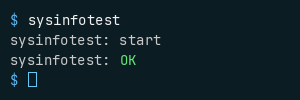
\includegraphics[width=0.55\textwidth]{images/sysinfo.png}
    \caption{Ảnh chụp kết quả thực thi chương trình kiểm thử \texttt{sysinfotest} trên QEMU}
    \label{fig:sysinfo_result}
\end{figure}

